%% ------------------------------------------------------------------------- %%
\chapter{Diferenças entre os dois mundos}
\label{cap:diferencas}

O manifesto ágil (apresentado na Caixa \ref{box:manifesto}, página
\pageref{box:manifesto}) é complementado por uma lista de 12
princípios traduzidos na Caixa \ref{box:principles}. Esses princípios
apresentam guias que norteiam os métodos ágeis na direção de algumas
práticas. Este Capítulo apresenta uma análise desses princípios sob o
ponto de vista de projetos de software livre com o objetivo de
identificar mais algumas semelhanças mas com destaque para as
diferenças entre as comunidades.

\begin{caixa}[htb]
  \begin{minipage}{\linewidth}
    \centering Seguimos esses princípios:

    \begin{itemize}
    \item Nossa maior prioridade é satisfazer o cliente através da
      entrega contínua e adiantada de software com valor agregado;
    \item Mudanças nos requisitos são bem-vindas, mesmo tardiamente no
      desenvolvimento.  Processos ágeis tiram vantagem das mudanças
      visando vantagem competitiva para o cliente;
    \item Entregar frequentemente software funcionando, de poucas
      semanas a poucos meses, com preferência à menor escala de tempo;
    \item Pessoas de negócio e desenvolvedores devem trabalhar
      diariamente em conjunto por todo o projeto;
    \item Construa projetos em torno de indivíduos motivados.  Dê a
      eles o ambiente e o suporte necessário e confie neles para fazer
      o trabalho;
    \item O método mais eficiente e eficaz de transmitir informações
      para e entre uma equipe de desenvolvimento é através de conversa
      face a face;
    \item Software funcionando é a medida primária de progresso;
    \item Os processos ágeis promovem desenvolvimento sustentável. Os
      patrocinadores, desenvolvedores e usuários devem ser capazes de
      manter um ritmo constante indefinidamente;
    \item Atenção contínua à excelência técnica e bom \textit{design}
      aumenta a agilidade;
    \item Simplicidade -- a arte de maximizar a quantidade de trabalho
      não realizado -- é essencial;
    \item As melhores arquiteturas, requisitos e \textit{designs}
      emergem de equipes auto-organizáveis;
    \item Em intervalos regulares, a equipe reflete sobre como se
      tornar mais eficaz e então refina e ajusta seu comportamento de
      acordo.
    \end{itemize}
  \end{minipage}
  \caption{Os 12 princípios do manifesto ágil}
  \label{box:principles}
\end{caixa}

A Seção \ref{sec:principles} apresenta a relação de princípios ágeis e
sua ligação com software livre para identificar os pontos principais
de diferença entre os movimentos. Em seguida, a Seção
\ref{sec:foss-over-agile} apresenta um pequeno resumo de um
\textit{workshop}\footnote{\url{http://submissions.agile2008.org/node/376}
  - Acessado em 16/03/2009} conduzido por Mary Poppendieck com
Christian Reis na Agile 2008. O \textit{workshop}, intitulado
\textit{``Open Source Meets Agile - What can each teach the other?''}
tinha como objetivo discutir práticas de sucesso em um projeto de
software livre que não eram encontradas em métodos ágeis. Desta forma,
os participantes poderiam compreender alguns princípios essenciais que
se aplicam a projetos de software livre e poderiam propor melhorias
aos atuais métodos ágeis.

Contrastando com este trabalho, a Seção \ref{sec:agile-improve-os}
apresenta as deficiências dos métodos ágeis mais conhecidos atualmente
no que diz respeito ao contexto de software livre. A Seção também
aborda como a criação de uma implementação de método ágil que lidesse
com o contexto de software livre poderia ajudar tanto projetos de
software livre quanto a comunidade de métodos ágeis.

\section{Princípios ágeis sob a ótica livre}
\label{sec:principles}

A lista de princípios ágeis apresenta alguns pontos de semelhança e
outros de diferença com software livre. As próximas Seções discutem
cada um dos princípios e seu uso em projetos de software livre.

\subsection[Satisfação do cliente]{Nossa maior prioridade é satisfazer
  o cliente através da entrega contínua e adiantada de software com
  valor agregado}

Esse princípio traduz para ações o valor de resposta a mudanças. Como
comentado no Capítulo \ref{cap:semelhancas}, projetos livres tem a
obrigação de atender aos pedidos de seus usuários caso contrário são
abandonados. Tem se tornado frequentes os projetos livres em que
existe uma periodicidade fixa para lançamento de novas versões como o
Eclipse\footnote{\url{http://www.eclipse.org/} -- Último acesso em
  28/10/2010} (que tem novas versões estáveis a cada ano e novas
versões instáveis a cada dois meses), a distribuição Linux
Ubuntu\footnote{\url{http://www.ubuntu.com} -- Último acesso em
  28/10/2010} (com versões estáveis a cada seis meses e versões
instáveis a cada dois meses) e o
OpenOffice\footnote{\url{http://www.openoffice.org} -- Último acesso
  em 28/10/2010} (cujas versões estáveis tem o objetivo de ser
lançadas a cada seis a oito meses e contar com três instáveis nesse
intervalo).

Esse ritmo permite obter feedback da comunidade sobre o andamento do
desenvolvimento. Para saber o que traz valor ao cliente, alguns
projetos também tem um sistema de rastreamento de problemas nos quais
os usuários podem ``votar'' nas funcionalidades mais importantes para
a próxima versão. O Bugzilla\footnote{\url{http://www.bugzilla.org} --
  Último acesso em 28/10/2010} é uma das ferramentas que permite esse
tipo de participação entre outras como
JIRA\footnote{\url{http://www.atlassian.com/software/jira/} -- Último
  acesso em 28/10/2010} e GitHub\footnote{\url{http://www.github.com}
  -- Último acesso em 28/10/2010}.

Dessa forma, muitos projetos de software livre abraçam esse princípio
e o incorporam em seus processos de desenvolvimento para poder atender
a sua comunidade.

\subsection[Aceitar as mudanças]{Mudanças nos requisitos são
  bem-vindas, mesmo tardiamente no desenvolvimento.  Processos ágeis
  tiram vantagem das mudanças visando vantagem competitiva para o
  cliente}

Nesse aspecto, projetos livres costumam adotar uma postura
extremamente ágil. Por conta da característica distribuída e
\textit{ad hoc} do software livre, é muito raro existir um momento de
coleta de requisitos pré-determinado. A coleta costuma acontecer de
forma contínua conforme usuários dos projetos enviam relatos de erros
e pedidos de funcionalidades ou conforme discussões acontecem nas
listas de correio eletrônico dos projetos.

Dessa forma, a questão de aceitar mudanças nos requisitos ``tarde'' no
desenvolvimento fica um pouco estranha. O único momento que pode ser
classificado como ``tarde'' num projeto com coleta contínua de
requisitos é uma vez que o requisito já estiver implementado. Mas, a
partir desse momento, mudanças no funcionamento passam a ser
descrições de erros (comportamento não esperado ou não desejado do
sistema).

A segunda parte do princípio afirma que essa resposta à mudança
deve se dar de forma a garantir um diferencial competitivo ao cliente,
isto é, as mudanças incorporadas devem ir na direção que atrairá mais
usuários. Em software livre, é muito difícil descobrir a curto ou
médio prazo o impacto de uma nova funcionalidade na base de usuários
já que a adoção e difusão dos projetos é relativamente lenta e pouco
controlada. Mas a longo prazo, apenas os projetos que conseguirem se
destacar permanecem.

\subsection[Entregas frequentes]{Entregar frequentemente software
  funcionando, de poucas semanas a poucos meses, com preferência à
  menor escala de tempo}

O freshmeat\footnote{\url{http://freshmeat.net/} -- Último acesso em
  28/10/2010} é um dos maiores site de notícias sobre novas versões de
projetos livres. O site está em atividade desde meados de 1990 e ainda
mantém seu histórico desde Fevereiro de 2001. Desta data até
05/01/2011, foram 214999 novas versões que formam uma média de 59.31
novas versões por dia.

Até 28/10/2010, eram 42800 projetos livres repertoriados e
controlados. Esses dados apontam uma média de 4.97 novas versões por
projeto ao longo de 3556 dias (9 anos e alguns meses).
Aproximadamente uma nova versão a cada dois anos por projeto.

Analisando os lançamentos efetuados entre 21/10/2001 e 28/10/2010, a
grande maioria dos projetos listados não tem uma frequência alta e
estável de lançamentos. A Figura \ref{fig:freshmeat} mostra a
distribuição de projetos por frequência de lançamento. É possível ver
que a grande maioria dos projetos demora mais de 6 meses para lançar
uma nova versão com apenas 17\% dos projetos lançando versões pelo
menos uma vez por semestre.

\begin{figure}
  \centering
  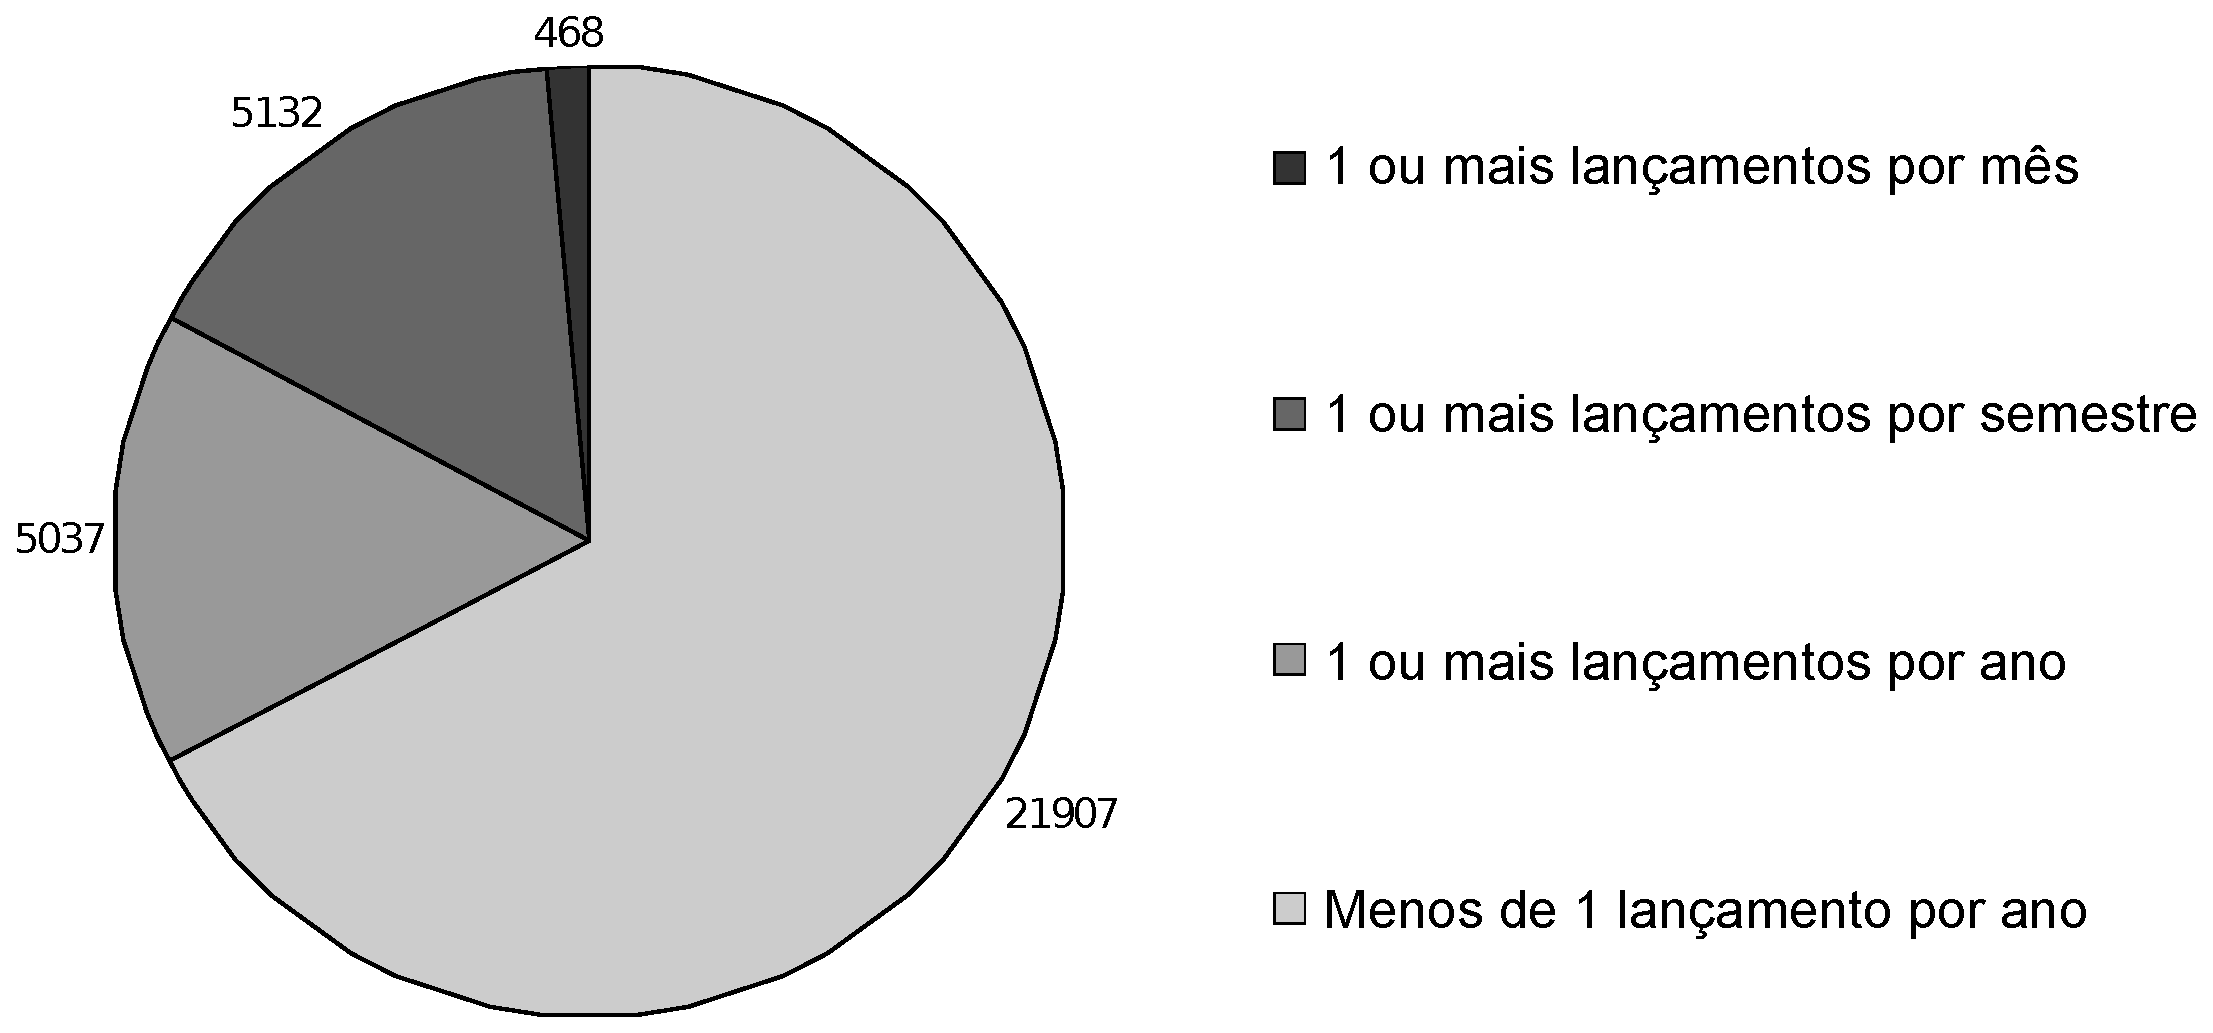
\includegraphics[scale=.3]{freshmeat}
  \caption{Quantidade de projetos por faixa de frequência de
    lançamento de acordo com o freshmeat.net}
  \label{fig:freshmeat}
\end{figure}

Desse ponto de vista, pode parecer que os projetos livres não seguem
muito esse princípio ágil. Mas deve-se também considerar que, entre
todos os projetos listados, alguns podem ter sido abandonados ou
simplesmente não avisaram o site de suas novas versões. Portanto é
provável que essa média não reflita a realidade para projetos de
software livre ativos.

Numa análise anual detalhada entre 2001 e 2010, descobre-se que o
número de lançamentos anuais assim como a quantidade de projetos com
pelo menos 2 lançamentos no ano tem caído desde 2004. A Figura
\ref{fig:freshmeat-by-years} mostra a evolução do número de releases
registrados no site por ano, a quantidade de projetos repertoriados e
a quantidade de projetos com, pelo menos 2 releases naquele ano.

\begin{figure}
  \centering
  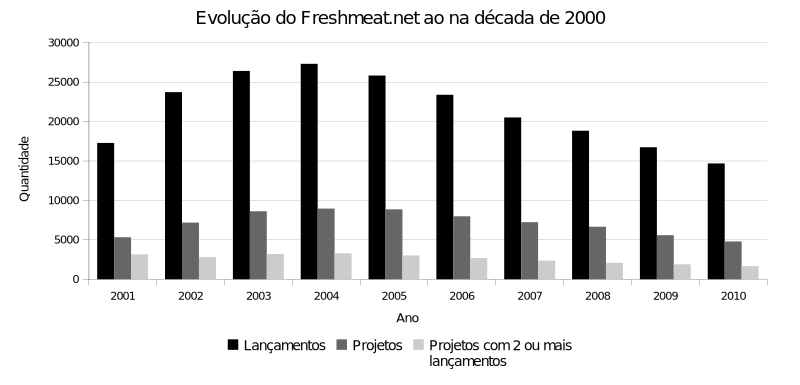
\includegraphics[scale=0.7]{freshmeat-by-years}
  \caption{Quantidade de lançamentos, projetos e projetos com 2 ou
    mais lançamentos por ano no Freshmeat.net}
  \label{fig:freshmeat-by-years}
\end{figure}

Não só o número de projetos e de lançamentos está diminuindo no
freshmeat.net mas a proporção de projetos com lançamentos
frequentes também. Em 2002, 38,91\% dos projetos registrado
anunciaram 2 ou mais lançamentos ao longo do ano. Em 2008, atingiu-se
o pico de meros 30,29\% dos projetos com 2 lançamentos anuais. Desde
então, a situação melhorou um pouco mas ainda é difícil prever se a
tendência é de aumento ou diminuição dessa proporção.

Além disso, vale notar que a escala de tempo para projetos livres
costuma ser um pouco maior do que em projetos proprietários que contam
com a dedicação em tempo integral dos membros da equipe. Desse ponto
de vista, algumas semanas de um projeto com dedicação integral podem
ser considerado equivalentes a alguns meses num projeto baseado em
voluntários.

De toda forma, esses resultados são indícios de que projetos livres
não seguem o princípios de entregar novas versões funcionais em
escalas de tempo pequenas. Esse é um ponto de possível melhora para
esses projetos.

\subsection[Trabalhar com pessoas de negócio]{Pessoas de negócio e
  desenvolvedores devem trabalhar diariamente em conjunto por todo o
  projeto}

Este é outro princípio em que o contexto comum de projetos livres
torna um pouco estranha a afirmação. Como Raymond diz: ``Todo bom
projeto de software começa com um desenvolvedor resolvendo um incômodo
pessoal'' \cite{Raymond1999}. Nesse caso, o especialista do negócio é
o próprio desenvolvedor o que faz com que seja impossível um trabalhar
sem o outro.

Desta forma, parece que qualquer projeto livre, para que evolua,
precisa abraçar esse princípio e garantir que sempre há algum
desenvolvedor envolvido que entenda o negócio que o projeto se propõe
a simplificar.

\subsection[Trabalhe com indivíduos motivados]{ Construa projetos em
  torno de indivíduos motivados.  Dê a eles o ambiente e o suporte
  necessário e confie neles para fazer o trabalho}

Para esse princípio parece mais justa a inversão de análise. Software
livre tem como premissa o envolvimento voluntário e, portanto,
motivado. A partir dessa motivação, os indivíduos reunem-se na
Internet (ambiente necessário) e começam a evoluir o projeto.

O movimento de software livre existe desde os anos 1970. No entanto, o
movimento só ganhou força na segunda metade da década de 1990. Esse
sucesso se deve, em grande parte, à difusão da Internet e ao aumento
do número de pessoas com acesso a um computador pessoal. Esse foi o
suporte essencial para o crescimento da comunidade de software
livre. Essas comunidades evoluem encima da possibilidade de se
auto-gerenciarem e evoluirem independentemente de fatores externos. A
tolerância a falhas no eco-sistema livre faz com que projetos que
encontram dificuldades demais na sua evolução falhem e, se o problema
for muito importante, serão atacados novamente no futuro até que seja
viável chegar a algum resultado prático.

É com base nesse princípio que surgiu e cresceu a
Wikipedia\footnote{\url{http://wikipedia.org} -- Último acesso em
  12/12/2010}. A Wikipedia é um exemplo de como um ambiente (a
Internet) com o suporte necessário (um
wiki\footnote{\url{http://wiki.org/wiki.cgi?WhatIsWiki} -- Último acesso em
  05/01/2011}) permite a indivíduos motivados (milhares de
contribuídores da Wikipedia) fazerem um trabalho incrível. Este
trabalho foi a principal causa para que a Microsoft encerasse, em
Abril de 2009, o desenvolvimento e distribuição da enciclopédia
Encarta. Em 2005, a revista Nature publicou um
artigo\footnote{\url{http://www.nature.com/nature/journal/v438/n7070/full/438900a.html}
  -- Último acesso em 05/01/2011} comparando a qualidade da Wikipedia
com a Encyclop{\ae}dia Britannica. O artigo chega à conclusão que os
artigos relacionados a ciência da Wikipedia são tão confiáveis quanto
os da Encyclop{\ae}dia Britannica.

\subsection[Conversa face a face]{O método mais eficiente e eficaz de
  transmitir informações para e entre uma equipe de desenvolvimento é
  através de conversa face a face}

Este é o princípio no qual está mais clara a separação entre software
livre e métodos ágeis. Pela natureza distribuída já discutida de
projetos livres, é praticamente impossível reunir os colaboradores de
um projeto num mesmo espaço físico. Por conta disso, o uso da conversa
face a face em projetos de software livre é praticamente impossível.

Como os resultados do questionário apresentado na Seção
\ref{sec:resp-floss}, o canal de comunicação mais usado e melhor
avaliado em projetos de software livre são listas de correio
eletrônico seguidos de canais IRC. Ambos são bem distantes de
conversas face a face. O primeiro não conta sequer com respostas
síncronas que é o único benefício apresentado no segundo. Com relação
a conversas face a face, ambos canais perdem a entonação da voz, as
expressões faciais, gesticulações além do contato visual.

Esse uso é tão difundido e aceito na comunidade de software livre que,
como apresentado na Seção \ref{sec:resp-floss}, canais IRC são até
melhor avaliados em termos de eficácia e eficiência do que as
conversas face a face pelos contribuidores. Percebe-se também que
outros canais mais próximos de conversas face a face tem um uso muito
raro o que mostra também uma falta de vontade de mudar a situação
atual.

Por tanto, pode-se dizer que há uma diferença real de valores nesse
aspecto. Métodos ágeis abrem mão da rastreabilidade das conversas em
prol de uma maior interação enquanto comunidades de software livre
favorecem esse histórico e essa rastreabilidade e consideram que os
canais menos fortes são suficientemente eficientes.

\subsection[Software funcionando]{Software funcionando é a medida
  primária de progresso}

Neste ponto, percebe-se talvez a maior ligação entre as duas
comunidades.

Projetos de software livre costumam ser avaliados de acordo com o
tamanho de sua comunidade e com relação à sua adoção. Desta forma, o
progresso de um projeto livre pode ser medido pela sua capacidade de
agregar uma comunidade importante e de ser adotado por muitos
usuários.

No entanto, é impossível ser adotado por usuários caso não exista um
programa em funcionamento. Além disso, de acordo com Riehle
\cite{Riehle2007}, as pessoas se envolvem com um projeto livre porque
este projeto as ajuda a resolverem seus problemas. Dito isso, não
basta ter algo em funcionamento, o programa precisa resolver os
problemas de seus usuários para atrair sua atenção e torná-los
colaboradores.

Sendo assim, parece razoável afirmar que o progresso de um projeto
livre só pode se dar com a liberação de software funcionando. Ou seja,
o progresso de um projeto livre pode ser medido pela sua capacidade de
entregar software funcionando.

\subsection[Ritmo sustentável]{Os processos ágeis promovem
  desenvolvimento sustentável. Os patrocinadores, desenvolvedores e
  usuários devem ser capazes de manter um ritmo constante
  indefinidamente}

No caso de projetos livres, o ritmo é ditado pelo envolvimento dos
voluntários de acordo com suas possibilidades. Dada a ausência de uma
entidade controladora da dedicação de cada parte, o ritmo de
comunidades de software livre é variado.

A proposta mais recente para atingir algo nesse sentido nas
comunidades livres é da ideia de lançamentos cadenciados. O Firefox e
o Ubuntu tem procurado lançar novas versões em intervalos de tempo
fixo e com escopo aberto. Isso significa que uma nova versão será
lançada numa data pré-determinada com as funcionalidades que estiverem
prontas e testadas.  Dessa forma, tira-se a pressão para conseguir
terminar determinado trabalho até uma certa data.

Infelizmente essa medida não garante que a equipe consiga manter um
ritmo constante. Especialmente considerando que muito desse trabalho é
realizado em tempo livre e sujeito à disponibilidade de cada um. Nesse
contexto, sustentável pode ter um sentido um pouco diferente do
sentido usado em métodos ágeis. Não é mais possível pensar em jornadas
de 40 horas e folga no planejamento. Apenas políticas que reduzam a
pressão existente para finalização de um determinado trabalho. A
cadência de lançamentos é uma prática que permite esse tipo de
solução.

\subsection[Excelência técnica]{Atenção contínua à excelência técnica
  e bom \textit{design} aumenta a agilidade}

Por construção, o movimento de software livre envolve pessoas
apaixonadas por desenvolvimento de software. Nesse aspecto, projetos
livres tendem a utilizar todo tipo de tecnologia.  Dia 18 de Agosto de
2010, os 10 projetos mais baixados do SourceForge.net reuniam 6
linguagens de programação diferentes (C, C++, Python, Javascript,
Delphi e Perl).

No dia 30/10/2010, o SourceForge.net listava em torno de 1600 projetos
com mais de 100.000 downloads. Desses projetos, 782 incluíam seu
código fonte em C, C++ ou Java na página do SourceForge.net.  Nessa
amostra, foi utilizada a ferramenta
Analizo\footnote{\url{http://analizo.org} -- Último acesso em 06/01/2011}
para levantar algumas métricas com relação ao código fonte desses
projetos.

Utilizando as propostas de valores de referências sugeridos por
Ferreira~\cite{Ferreira2009}, foi realizada uma análise dos projetos
com relação à qualidade de seu \textit{design}. As métricas analisadas
foram:
\begin{enumerate}
\item Média de Conexões Aferentes,
  \label{metric:acc}
\item Fator de Acoplamento Total e
  \label{metric:cof}
\item Máxima Profundidade da Árvore de Herança,
  \label{metric:dti}
\item Moda da Ausência de Coesão em Métodos,
  \label{metric:lcom}
\item Média do Número de Atributos Públicos de uma Classe,
  \label{metric:npa}
\item Média do Número de Métodos Públicos de uma Classe,
  \label{metric:npm}
\end{enumerate}

No que diz respeito à métrica \ref{metric:acc}, Ferreira estipula
valores abaixo de 1 como valores bons, até 20 como valores regulares e
acima de 20 como valores ruins. Com essas referências, apenas 15\% dos
projetos possui uma média de conexões aferentes considerada boa. No
entanto, todos os outros 77\% tem uma média abaixo de 5 e nenhum tem
média acima de 20. Isso nos indica que, apesar de poucos projetos
estarem no nível bom, a maioria deles está próximo do valor de
referência. Esse resultado nos indica uma qualidade razoável dos
projetos livres.

A métrica \ref{metric:cof} usa como parte do seu cálculo o resultado
da métrica \ref{metric:acc}. No entanto, de acordo com os valores de
referência apresentados por Ferreira, 57\% do projetos tem fatores de
acoplamento considerados bons enquanto 34\% tem valores regulares e 9\%
tem valores ruins. Com esses resultados parece que uma porção bem
maior do projetos livres tem um cuidado considerável em manter sua
arquitetura desacoplada.

Para a métrica \ref{metric:dti}, Ferreira apresenta uma média de 1,68
como referência. Dessa forma, o ideal sugerido é que o valor máximo da
métrica seja 2. Nos projetos avaliados, 69\% atingem essa meta
enquanto 19\% tem árvores com o dobro da profundidade. Nesse caso, os
resultados são um pouco piores. Com quase 20\% dos projetos com uma
árvore de herança profunda, há um indício de um pequeno desleixo na
questão da arquitetura em projetos livres.

Com relação à métrica \ref{metric:lcom}, Ferreira apresenta uma
ausência de coesão 0 como uma medida boa (já que, em seu estudo, 50\%
das classes tinham 0 de ausência de coesão) enquanto valores entre 0 e
20 são regulares. Para atingir valores semelhantes, olha-se a moda da
métrica para observar os projetos com mais de 50\% das classes com
determinado valor para a métrica. Nessa análise, percebe-se que 39\%
dos projetos atingem a meta enquanto o resto concentra-se abaixo de 20
(valor considerado razoável). Essa métrica tem resultados semelhantes
aos da métrica \ref{metric:acc} e indica uma qualidade, ainda que não
boa, bem próxima disso.

O número de atributos públicos (métrica \ref{metric:npa}) de uma
classe aponta uma exposição excessiva (se for alto) de detalhes de
implementação. Ferreira diz que 75\% das classes analisadas em seu
estudo não possuiam nenhum atributo público enquanto a maioria do
restante tinha menos de 8 atributos públicos. Sendo assim, os valores
sugeridos são de nenhum atributo público para uma boa arquitetura, até
8 atributos públicos como regular e mais do que isso sendo ruim. Na
média dos projetos analisados, foram considerados bons, os projetos
que atingiam uma média inferior a 1 atributo público por classe e,
ruins, os projetos com média acima de 8 atributos. Nesse caso,
obtem-se 21\% de projetos bons, 24\% de projetos ruins e 55\% de
projetos regulares. Esse é mais um ponto que indica uma falta de
preocupação com a qualidade do \textit{design} do projeto.

Por fim, o número de métodos públicos (métrica \ref{metric:npm}) de uma
classe dá indícios com relação à quantidade de responsabilidades da
classe. Ferreira aponta valores de referência sendo bom para até 10
métodos públicos, regular entre 10 e 40 e ruim acima de 40 métodos
públicos. Com esses valores, 77\% dos projetos analisados são
considerados bons enquanto 21\% são regulares e meros 1\% são
ruins. No entanto, 52\% dos projetos considerados bons tem uma média
acima de 5 métodos públicos o que indica que apesar da métrica ser
cumprida, ela está próxima do limite estipulado.

Dessa forma, os projetos analisados dão indícios de que, em projetos
de software livre de sucesso, existe uma atenção considerável dada à
qualidade técnica e ao \textit{design}. No entanto, algumas métricas
indicam que os projetos estão frequentemente no limiar aceitável e
fazem o mínimo necessário para conseguirem se manter numa situação
boa. A adoção de refatorações frequentes poderia ajudar a resolver os
probleminhas de profundidade da árvore de herança assim como dos
atributos públicos.

\subsection[Simplicidade é essencial]{Simplicidade -- a arte de
  maximizar a quantidade de trabalho não realizado -- é essencial}

Software livre se apoia no princípio da quantidade para obter
qualidade. Isso significa que muitos projetos são criados, evoluídos e
mantidos por um tempo mas abandonados em seguida.

De acordo com o
FLOSSMETRICS\footnote{\url{http://www.flossmetrics.org} -- Último
  acesso em 29/10/2010}, em 2007, apenas 9.2\% dos projetos do
SourceForge.net\footnote{\url{http://www.sf.net} -- Último acesso em
    29/10/2010} eram considerados ativos. Onde ativos significa que
tiveram alguma liberação de arquivos nos últimos 6 meses e houve
registro de atividade no site nesse período. Isso aponta que a grande
maioria dos projetos que foram iniciados não tiveram
continuidade. Nesse sentido, existe MUITO trabalho realizado que é
pouco aproveitado.

Por outro lado, ainda não tem-se acesso a nenhuma ferramenta que
análise projeto a projeto e avalie se as funcionalidades
implementadas são realmente necessárias. Logo, não é possível
determinar se os projetos livres adotam o princípio da simplicidade.

\subsection[Equipes auto-organizáveis]{As melhores arquiteturas,
  requisitos e \textit{designs} emergem de equipes auto-organizáveis}

A teoria com relação a esse princípio é a mesma em ambas
comunidades. Projetos livres emergem da vontade de programadores que
se auto-organizam para desenvolver um programa.

No que diz respeito aos requisitos, de acordo com Eric Raymond,
projetos livres surgem de problemas enfrentados pelos seus próprios
desenvolvedores. Neste caso, os requisitos vem dos próprios
desenvolvedores o que simplifica amplamente o problema de
entendimento.

Com relação às arquiteturas e \textit{designs}, é difícil avaliar de
forma genérica quão bons são as soluções implementadas em projetos
livres. Alguns projetos livres apresentam arquiteturas que resistiram
ao tempo e viraram referências como os projetos Ruby on Rails,
Firefox, Eclipse e o Kernel do Linux. No entanto, isso não é
suficiente para afirmar que as comunidades de software livre
desenvolvem boas arquiteturas e \textit{designs}. Pode-se afirmar, no
entanto, que, pelo fato das equipes serem intrinsicamente
auto-organizáveis, elas geram as melhores arquiteturas que poderiam
gerar já que toda decisão deve ser discutida por todos os envolvidos.

\subsection[Refletir regularmente]{Em intervalos regulares, a equipe
  reflete sobre como se tornar mais eficaz e então refina e ajusta seu
  comportamento de acordo}

Aqui está uma das diferenças mais claras entre métodos ágeis e
projetos livres. A capacidade e costume de juntar a equipe para pensar
sobre o processo de desenvolvimento dificilmente é possível
considerando que o modelo de desenvolvimento é assíncrono, distribuído
e voluntário.

\section{Princípios do Software Livre interessantes em Métodos Ágeis}
\label{sec:foss-over-agile}

Dada a avaliação anterior, é possível perceber que existem algumas
diferenças consideráveis no que diz respeito aos princípios
compartilhados entre as duas comunidades. Essa seção apresenta alguns
conceitos que são exclusivos ao ambiente de desenvolvimento de
software livre mas que poderiam trazer benefícios para métodos ágeis
num contexto distribuído. Esses conceitos foram coletados durante um
\emph{workshop} organizado por Mary Poppendieck na Agile 2008 em
Toronto com Christian Reis.

Reis é um desenvolvedor Brasileiro de software livre que trabalha para
a Canonical Inc. no desenvolvimento do LaunchPad
\footnote{\url{http://launchpad.net/} - Último acesso 28/10/2010}, o
projeto de gerenciamento de software para a distribuição Linux
Ubuntu. O \emph{workshop} teve início com a apresentação de Reis sobre
como o LaunchPad é desenvolvido. Três pontos essenciais foram
levantados durante a discussão que deu sequência à apresentação. O
primeiro (Subseção \ref{subsec:commiter}) descreve e discute o papel
de \emph{commiter}.  O segundo (Subseção \ref{subsec:publicity})
apresenta os benefícios de seguir um processo de desenvolvimento que
seja público e transparente.  Por fim, o último (Subseção
\ref{subsec:crossrev}) aborda o sistema de revisão cruzada dos
sistemas que é usado para garantir a comunicação e a clareza do
código.

\subsection{O papel do \emph{Commiter}}
\label{subsec:commiter}

Parte do valor que foi identificado no software livre foi o papel do
\emph{commiter}. Como esse papel tem uma relação relativamente
complicada com métodos ágeis, essa subseção será divida em quatro
partes. A primeira descreve o que é um \emph{commiter}. A segunda
apresenta como esse papel é distribuído em métodos ágeis. A terceira
aborda as diferenças e semelhanças entre a revisão realizada durante a
programação em pares e a revisão feita pelo \emph{commiter}. Por fim,
a quarta apresenta as sugestões de adaptação desse papel em métodos
ágeis.

\subsubsection{O que é um \emph{commiter}}

Um \emph{commiter} é uma pessoa que tem direito de adicionar,
modificar e remover código fonte ao ``ramo''\footnote{Um ramo
  (\emph{branch}) de um repositório é uma ramificação da estrutura de
  diretórios que guarda os arquivos} principal do repositório de
controle de versões. O ``ramo'' principal é a parte do código que será
empacotada para formar uma nova versão do programa. Aos olhos da
comunidade do software, o \emph{commiter} é uma pessoa confiável muito
qualificada para avaliar a qualidade do código fonte. Este é o meio
encontrado pelas comunidades de software livre para revisar a grande
maioria do código fonte de forma a reduzir a quantidade de erros e
melhorar a clareza do código.

A maioria dos projetos de software livre tem um grupo muito pequeno de
\emph{commiters}. Frequentemente o líder do projeto é o único
\emph{commiter} e todos os \emph{patches} devem passar por sua
aprovação. De acordo com Riehle \cite{Riehle2007}, existem três níveis
na hierarquia tradicional de um projeto de software livre.
\begin{itemize}
\item O primeiro nível é o de usuário.

  Usuários têm o direito de usar o programa, relatar problemas e pedir
  funcionalidades.
\item O segundo nível é o de contribuidor.

  A promoção entre o primeiro e o segundo nível é implícita. Ela
  acontece quando um \emph{commiter} aceita os \emph{patches} do
  usuário e os envia ao repositório de código no ``ramo''
  principal. Normalmente, ninguém sabe dessa promoção, com exceção do
  \emph{commiter} e do contribuidor.
\item O terceiro papel é o de \emph{commiter}.

  Neste nível, a transição é explícita. Contribuidores e
  \emph{commiters} demonstram apoio a uma determinada pessoa e
  reconhecem publicamente a qualidade geral de seu trabalho. Por isso,
  atingir o nível de \emph{commiter} é um feito valioso que significa
  que essa pessoa produz código de ótima qualidade e está realmente
  envolvida com o desenvolvimento do projeto.
\end{itemize}

\subsubsection{O papel do \emph{commiter} em métodos ágeis}

Métodos ágeis delegam o papel do \emph{commiter} para cada um dos
desenvolvedores da equipe. No \emph{workshop} sugeriram que alguma
forma de controle no ``ramo'' principal de um projeto ágil poderia
melhorar ainda mais a simplicidade do código fonte do aplicativo de
produção.

Na maioria dos métodos ágeis, uma equipe deveria ter um líder (um
\emph{Scrum Master} em Scrum, um \emph{coach} em XP, etc...)  que é
mais experiente naquele método ágil que o resto da equipe. O líder da
equipe é responsável por lembrar a equipe de se ater às práticas
escolhidas. Ele também deve ajudar a equipe a resolver os problemas
encontrados e idealmente, transformar todos os membros da equipe em
possíveis líderes de forma a tornar-se ``inútil''.

Para cumprir essa função, o líder não precisa obrigatoriamente ter
conhecimentos técnicos apurados. No entanto, uma equipe de
desenvolvimento costumeiramente precisa de ajuda do ponto de vista
técnico em alguma parte de seu trabalho. Alguns dos problemas
levantados por uma equipe podem ser causados por decisões ou por
dificuldades técnicas. Neste caso, se o líder não tiver conhecimento
técnico, ele pode encontrar dificuldades para cumprir sua função. Para
resolver este problema, é comum que o líder tenha a ajuda de um
consultor técnico que pode ser um membro da equipe ou uma pessoa de
fora.

Se este consultor técnico for um membro da equipe, ele tem,
indiretamente, a responsabilidade de fazer com que a equipe mantenha
uma boa qualidade de código. Pensando assim, o responsável técnico tem
a função de \emph{commiter} do projeto mas realiza seu trabalho
lembrando aos programadores de que seu código deve estar sempre
legível, claro e com testes passando.

\subsubsection{Semelhanças e diferenças da revisão}

O papel ativo de revisor que o \emph{commiter} tem em projetos de
software livre é encontrado no copiloto de uma dupla de programação em
pares. Note, no entanto, que a revisão de código realizada durante a
programação em pares tem como objetivo principal a redução de erros e
não é obrigatoriamente eficiente no aumento da clareza do código. Isso
se dá porque, quando um par trabalha em uma tarefa, ambas pessoas
mergulham em um determinado trecho de código e criam juntas uma linha
de pensamento. Para ambos os envolvidos, o tal trecho de código pode
ser muito claro graças ao contexto e à linha de pensamento que eles
criaram. Mas, para alguém que não acompanhou essa linha, o código pode
ser muito complexo se ele não deixar indícios do raciocínio que deve
ser seguido.

A revisão feita pelo \emph{commiter} dificilmente será mais eficiente
que a do par para reduzir a quantidade de erros já que o revisor
costuma ter menos tempo para pensar sobre o problema e entender os
possíveis casos envolvidos. Enquanto o par que trabalhou no código
teve exatamente este objetivo. No entanto, o \emph{commiter} traz um
olhar fresco ao código que é muito mais semelhante ao olhar de um
desenvolvedor qualquer no futuro. Deste ponto de vista, é mais
provável que o revisor questione o código de forma semelhante àquela
que outra pessoa no futuro faria. Sendo assim, o \emph{commiter} pode
evitar os principais problemas relacionados à clareza do código
produzido.

De qualquer forma, o trabalho de revisão tem duas consequências
diretas e evidentes. A primeira é de que o tempo necessário para que
uma mudança seja incorporada ao ``ramo'' principal do código aumenta
consideravelmente já que, tipicamente, são necessárias algumas
conversas entre o revisor e os autores do código. A segunda é que o
trabalho do revisor, se ele for único, é considerável já que ele deve
ler todo código que deve ir para o ``ramo'' principal, tentar
entendê-lo e expressar suas dúvidas aos autores.

\subsubsection{Sugestões para adaptar o papel aos métodos ágeis}

Considerando os pontos apresentados no fim da seção anterior, dar o
papel de \emph{commiter} ao consultor técnico de uma equipe ágil
significaria criar um gargalo de incorporação de código. A Teoria das
Restrições \cite{goldratt84} afirma que deve-se eliminar os gargalos
para maximizar a produtividade de uma equipe.

Sendo assim, a proposta é manter um pequeno conjunto de
desenvolvedores da equipe como \emph{commiters} e fazer o papel
circular entre os membros da equipe. Dessa forma, além de diminuir o
gargalo, também reduz-se o ``\textit{truck
  factor}''\cite{Williams2002} (ou ``fator caminhão'') da
equipe. ``Fator caminhão'' é uma expressão para expressar a quantidade
de membros da equipe que precisam se ausentar do projeto para que ele
pare. Quanto maior esse número, maior o conhecimento difundido pelos
membros da equipe e menor o risco desse projeto parar.

O papel de \emph{commiter} é crítico em um projeto já que a ausência
de pessoas realizando esse papel impede o código do projeto de ir para
produção. Dessa forma, é importante aumentar o número de
\emph{commiters} num projeto sem, no entanto, banalizá-lo ao ponto de
que a revisão cruzada não aconteça mais. Outra possibilidade é a de
distribuir o papel entre todos os membros da equipe mas forçar que
exista uma revisão aprovada por um terceiro membro da equipe (além do
par que desenvolveu a funcionalidade) para que o \emph{commit} seja
enviado ao ``ramo'' principal.

Ambas soluções aumentam o conjunto de \emph{commiters}, distribuem
mais o conhecimento entre a equipe e reduzem a aparente concentração
de poder desse papel. Elas também permitem que aqueles que foram
\emph{commiters} possam, por sua vez, serem autores de alguns trechos
de código que passarão por avaliação de outros. Desta forma, toda a
equipe passa a entender o valor de cada um dos papéis e entende melhor
como escrever código que seja claro para um revisor.

É necessário, no entanto, tomar cuidado para que isso não se torne um
fardo para a equipe e evite que ela responda às mudanças que se
apresentarem. Em equipes muito pequenas, a rotação frequente de pares
resolve o problema da difusão do conhecimento. Nesse contexto, o
problema de integridade conceitual descrito por Frederick Brooks
\cite{Brooks1975-mmme} é menor o que torna a revisão menos crítica.

\subsection{Resultados públicos}
\label{subsec:publicity}

Outro ponto importante da discussão foi a divulgação pública de todos
os resultados relacionados ao projeto. De acordo com Reis, programas
proprietários também podem se beneficiar de um sistema de rastreamento
de erros público e da publicação dos resultados dos testes
automatizados. Para abraçar os benefícios dessas práticas é necessário
expor alguns detalhes de código. Disponibilizar esses resultados
publicamente encoraja os usuários a participar do processo de
desenvolvimento já que eles entendem como e quando o programa é
melhorado.

Em métodos ágeis, o resultado dos testes e a lista fornecida pelo
sistema de rastreamento de erros são informações muito importantes
para a equipe de desenvolvimento. Apesar disso, nenhum métodos afirma
explicitamente que o cliente e os usuários deveriam estar em contato
direto com essas ferramentas.

É senso comum em métodos ágeis que o cliente deveria ser parte da
equipe de desenvolvimento. Como a equipe deve estar sempre em contato
com essas ferramentas, pode-se interpretar que o cliente deveria usar
a ferramenta de forma semelhante ao resto da equipe. Infelizmente, a
maioria das ferramentas usadas são muito rudimentares do ponto de
vista de um cliente não técnico já que poucas delas se preocupam em
atribuir um significado de negócios aos resultados.

Algumas iniciativas\footnote{RSpec - \url{http://rspec.info/} - Último
  acesso em 28/10/2010}$^{, }$\footnote{JBehave -
  \url{http://jbehave.org/} - Último acesso em 28/10/2010}
relacionadas aos testes já existem ligadas ao movimento de
Desenvolvimento Dirigido pelo Comportamento (\emph{BDD - Behaviour
  Driven Development}) \cite{North2006} para produzir melhores
relatórios.

Mas a divulgação pública de informações relacionadas ao projeto não se
restringe aos erros ou aos testes. Nas comunidades de software livre,
as discussões entre os membros do projeto e até as discussões com
pessoas de fora do projeto sempre são guardadas no histórico da lista
de correio eletrônico usada. Discussões fora dessa lista são
fortemente desencorajadas já que elas impedem outras pessoas de
contribuir com comentários e ideias. Os históricos das listas ajudam a
construir uma documentação para futuros usuários assim como criar um
rápido sistema de \emph{feedback} para novatos.

Além disso, manter o histórico da lista também inibe atitudes
desrespeitosas já que todas as discussões são salvas e guardadas para
acesso futuro. Desta forma, os participantes costumam manter o
respeito (que é importantíssimo para o sucesso de qualquer projeto)
entre eles e com novatos. Aqui percebe-se mais uma forte ligação com
métodos ágeis. Respeito é um dos cinco valores da Programação Extrema
\cite{XP02}.

A rastreabilidade é um dos pontos fracos dos métodos ágeis. A maioria
dos métodos sugere que o projeto do software (\emph{design}) evolua
com o tempo conforme as necessidades. Essa evolução deveria fluir
naturalmente dos quadros brancos ou \emph{flip charts}. O problema com
essa abordagem é que quadro brancos são apagados e \emph{flip charts}
são reciclados.  Mesmo quando estes são guardados de alguma forma
(fotos, transcrições ou até mesmo no código), as discussões que
levaram à solução são perdidas.

A fala é uma forma muito eficiente de comunicação mas também muito
efêmera. Mesmo quando uma conversa é gravada, é difícil buscar
informações sobre algum trecho da discussão. Correios eletrônicos são
muito menos eficientes para a comunicação mas têm um grande ganho na
facilidade de busca. Num curto prazo, é evidente que a conversa é
muito mais eficiente para transmitir ideias que a escrita,
especialmente em equipes pequenas. No entanto, num médio ou longo
prazo, os ganhos da comunicação escrita podem superar (como eles o
fazem em projetos livres) as perdas.

Em suma, métodos ágeis poderiam tornar seus resultados públicos da
seguinte forma. Existem várias informações que podem ser obtidas
automaticamente como relatórios de execução dos testes, estado do
processo de contrução do aplicativo, número de erros em aberto etc.
O sistema de build automático e de integração contínua poderia
publicar todas essas informações automaticamente em uma página
relacionada ao projeto. No que diz respeito às conversas, um esforço
pode ser realizar para incluir trechos de conversa e links em
mensagens de \textit{commits}. E, com ajuda da ferramenta de gestão de
projeto, os \textit{commits} podem ser exibidos de forma rica (com
imagens, links etc.) numa linha do tempo relacionada aos trabalhos
realizados.

\subsection{Revisão cruzada}
\label{subsec:crossrev}

O terceiro ponto que Reis apresentou foi bem específico ao
LaunchPad. Como o LaunchPad é uma plataforma usada por outras equipes
para que elas desenvolvam seus próprios projetos, quando há uma
mudança na Interface de Programação da Aplicação (\emph{API -
  Application Programming Interface}), um membro de uma equipe externa
que usa o programa (preferenciamente uma pessoa diferente a cada vez)
deve revisar a mudança da interface e os motivos que levaram a
ela. Essa mudança não pode ser enviada ao ``ramo'' principal do
repositório a não ser que o revisor externo a aprove. Essa prática é
conhecida como revisão cruzada das mudanças de API ou, simplesmente,
uma revisão cruzada.

Essa prática resolve alguns problemas de uma só vez. O papel do
\emph{commiter} resolve o problema da revisão de código que os métodos
ágeis atacam com a programação em pares. A revisão cruzada garante que
a mudança da interface é aprovada pelos usuários assim como os
desenvolvedores.

Ela também garante uma melhora considerável sobre aquela API já que a
conversa entre o desenvolvedor do projeto e o usuário é arquivada pela
lista de correio eletrônico. Desta forma, futuros usuários ou mesmo
outros usuários atuais podem ler e entender porque a API mudou e como
usá-la quando for necessário. Também fica mais fácil realizar mudanças
no futuro e simplificações já que fica claro o que aquela API está
querendo permitir e se aquilo ainda faz sentido nas novas versões.

Por fim, a revisão cruzada também ajuda a envolver o cliente nas
decisões de arquitetura da solução e garante que ele está de acordo
com as mudanças realizadas. Com isso, é mais fácil identificar um
possível problema de requisitos e corrigi-lo antes que eles sejam
implementados na base principal de código. Obviamente, esta prática só
pode se aplicar até um certo nível quando o usuário não tem
conhecimento técnico. Uma revisão externa pode ajudar a garantir a
clareza da API e a documentar as mudanças mas ela não vai identificar
problemas de requisitos se o revisor não for um cliente ou usuário.

% TODO Procurar trabalhos do Sutherland sobre MA distribuídos

\section{Contribuições de Métodos Ágeis no Software Livre}
\label{sec:agile-improve-os}

Da mesma forma que a comunidade de software livre possui soluções para
problemas comuns em seus contextos, métodos ágeis também evoluiram
algumas soluções que podem ser utilizadas em outros contextos. Em
especial, para algumas das dificuldades encontradas pelas comunidades
de software livre, existem práticas ágeis cujo objetivo é reduzir o
impacto dessas dificuldades.

A maioria desses problemas específicos de software livre são
relacionados a dificuldades de comunicação causados pela quantidade de
pessoas envolvidas no projeto, separação física e sua diversidade de
conhecimentos e culturas. Apesar desses fatores serem levados ao
extremo em projetos de software livre, equipes de métodos ágeis
distribuídas encontram alguns dos mesmos problemas
\cite{Sutherland2007,Maurer2002}.

Como Beck sugere \cite{Beck2008}, ferramentas podem melhorar a adoção
e o uso de práticas ágeis e, dessa forma, melhorar o processo de
desenvolvimento. Uma quantidade considerável de trabalho já foi
realizado na questão de ferramentas da programação em pares
distribuída\footnote{\url{http://sf.net/projects/xpairtise/} - Último
  acesso: 28/10/2010}$^{,}$
\footnote{\url{https://www.inf.fu-berlin.de/w/SE/DPP} - Último acesso:
  26/09/2009}$^{,}$ \footnote{\url{http://sangam.sourceforge.net/} -
  Último acesso: 28/10/2010} e estudos a respeito \cite{Nagappan2003}
mas pouco tem sido produzido para apoiar outras práticas. Como o
problema está relacionado à comunicação, algumas práticas de métodos
ágeis são relevantes. As próximas subseções vão apresentar essas
práticas e as ferramentas sugeridas para facilitar a adoção de métodos
ágeis na comunidade de software livre.

\subsection{Ambiente informativo}
\label{subsec:inform-worksp}

Essa prática sugere que uma equipe de métodos ágeis deveria trabalhar
num ambiente que provê informações relacionadas ao trabalho. Beck
\cite{XP01} atribui um papel específico, o de acompanhador
(\emph{tracker}), para uma pessoa (ou algumas pessoas) que deve manter
essa informação disponível e atualizada para a equipe. Com equipes
concentradas em um mesmo local físico, o acompanhador normalmente
coleta métricas \cite{Sato2007} automaticamente e seleciona algumas
delas para apresentá-las no ambiente. A maioria das métricas objetivas
são relacionadas ao código fonte enquanto as métricas subjetivas
costumam depender da opinião dos membros da equipe.

A coleta destes dados não é uma tarefa árdua mas normalmente consome
um tempo considerável e não agrega um benefício imediato ao projeto. É
provalvemente esse o motivo para a falta de métricas ou dados
atualizados em páginas de projeto de software livre. Uma ferramenta
que poderia melhorar esse cenários seria um sistema baseado em
\emph{plug ins} com um conjunto inicial de métricas e uma forma de
criar e apresentar novas métricas. Essas ferramentas deveriam estar
disponíveis em incubadoras de software livre de forma a permitir que
os projetos possam facilmente ligar seus repositórios e páginas à
ferramenta.

O projeto QualiPSo\footnote{\url{http://www.qualipso.org} -- Último
  acesso em 29/10/2010} possui uma área de trabalho inteiramente
dedicada ao desenvolvimento e exploração de dados relacionados a essa
prática. A área de ``Gestão de Informação'' tem como objetivo prover
ferramentas e indicações de como aproveitar as informações geradas
durante a vida de um projeto para aumentar a confiabilidade e
qualidade do mesmo. Os resultados dessa área de trabalho tem como
objetivo serem integrados pelo portal de projetos livres do QualiPSo
de forma a prover o uso de todos esses benefícios aos projetos lá
hospedados.

\subsection{Histórias}
\label{subsec:stories}

Com relação ao sistema de planejamento, XP sugere que os requisitos
deveriam ser coletados em cartões de histórias. O objetivo disto é
reduzir a quantidade de esforço necessário para descobrir qual é o
próximo passo a ser tomado e tornar fácil modificar essas prioridades
ao longo do tempo. Projetos de software livre normalmente guardam seus
requisitos em sistemas de rastreamento de erros. Quando se identifica
a falta de uma funcionalidade, cadastra-se um erro que deveria ser
corrigido e as discussões e sugestões de mudanças são enviadas para
aquele ``erro''. O problema com essa abordagem é que mudar a
prioridade desses ``erros'' e organizar um planejamento consome muito
tempo e se baseia em fatos que podem mudar com o tempo (tal como
``essa versão deveria resolver erros com prioridade acima de
8''). Também é muito difícil obter uma visão geral dos requisitos.

Descobrir as principais prioridades para a equipe rapidamente e ser
capaz de mudar essas prioridades de acordo com o \emph{feedback} é uma
das chaves para desenvolver software funcional. Para poder atingir
esse objetivo, uma ferramenta deveria ser desenvolvida para permitir
que erros sejam vistos como objetos móveis num quadro de planejamento
de versão. Para permitir que a comunidade envolvida possa colaborar
com seu conhecimento, a ferramenta deveria apresentar a prioridade do
erro assim como seu conteúdo de uma forma similar ao dos artigos da
Wikipedia \cite{Surowiecki2004,Tapscott2006,Benkler2006}.

\subsection{Retrospectiva}
\label{subsec:retrospect}

Essa prática sugere que a equipe deveria se juntar num ambiente físico
periodicamente para discutir o andamento do projeto. Existem dois
problemas nessa prática em equipes de software livre. O primeiro é de
que todos os membros da equipe devem estar presentes ao mesmo tempo no
mesmo lugar. O segundo é fazer com que a equipe interaja de forma
coletiva para apontar os problemas e as soluções que surgiram durante
o período avaliado. Uma das formas mais comuns para ajudar os
participantes a realizar esse trabalho é apresentar uma linha temporal
e pedir para que eles façam anotações sobre os eventos que ocorreram
nesse período. Isso os ajuda a relembrar os acontecimentos e entender
porque as coisas aconteceram da forma que aconteceram como pode ser
visto na Figura \ref{fig:timelineretro}.

\begin{figure}[htb]
  \begin{minipage}[t]{0.5\linewidth}
    \centering
    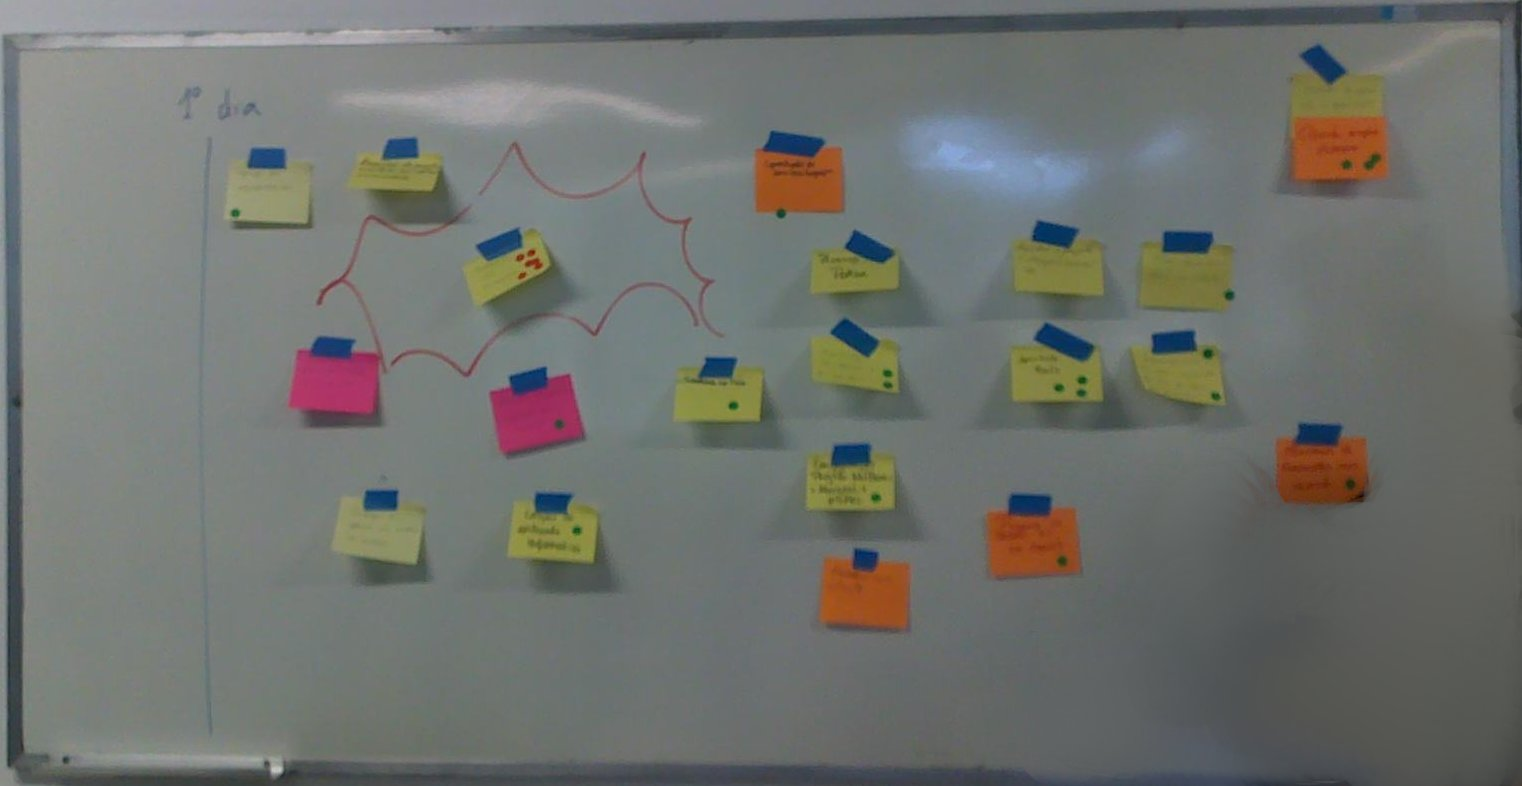
\includegraphics[width=\linewidth]{timeline-retro1}
  \end{minipage}
  \begin{minipage}[t]{0.5\linewidth}
    \centering
    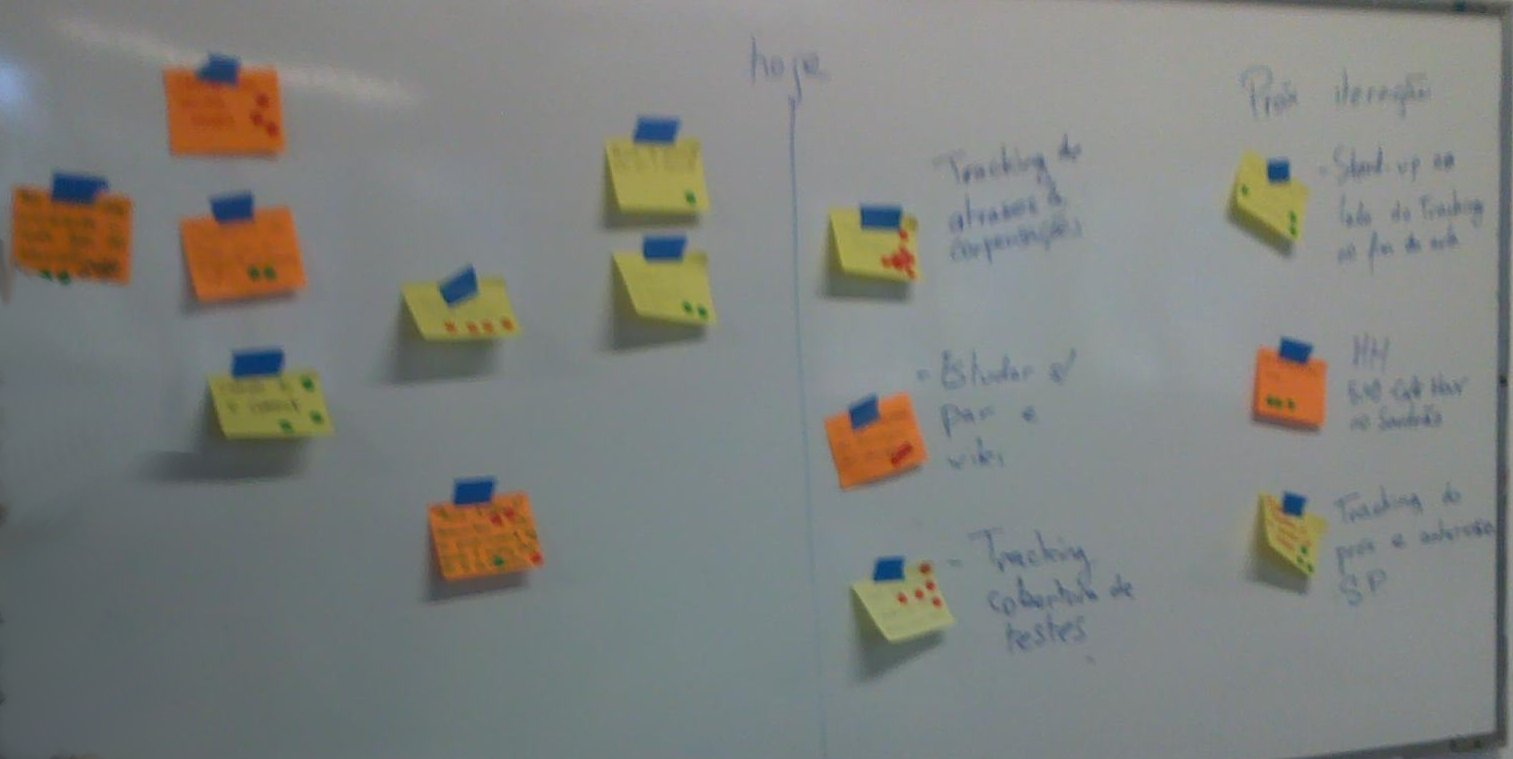
\includegraphics[width=\linewidth]{timeline-retro2}
  \end{minipage}
  \caption{Um exemplo de uma retrospectiva com linha do tempo}
  \label{fig:timelineretro}
\end{figure}

Quando a equipe está reunida em um único local físico, basta juntar a
equipe numa sala de reunião com uma linha do tempo grande na parede e
distribuir papéis coloridos que eles possam colar em ordenadas
escolhidas. A sugestão para equipes de software livre é desenvolver
uma ferramenta baseada na Internet para permitir que essas anotações
sejam feitas numa linha do tempo virtual associada ao código
fonte. Dessa forma, mensagens de integração de código poderiam conter
a anotação que seria automaticamente exibida na linha do tempo. Além
disso, a equipe poderia anotar a linha do tempo de forma assíncrona
para permitir comentários posteriores. O líder da equipe poderia
ocasionalmente gerar um relatório para todos os membros da equipe além
de exibir a linha do tempo no ambiente informativo.

Resta ainda conseguir fazer com que a equipe utilize as informações
coletadas para sugerir mudanças no processo para melhorar sua situação
atual. Numa retrospectiva, é muito importante que os membros da equipe
é que apontem os problemas que desejam resolver e como
resolvê-los. Também é essencial que todos aceitem que os problemas
escolhidos para serem tratados são os mais importantes e que concordem
com as propostas de soluções. Para atingir esses objetivos, é
necessário que a equipe converse entre si. No caso de um projeto
livre, isso significa que, de tempo em tempos, a equipe deveria se
reunir em seu canal de comunicação e ter essa conversa com base na
linha do tempo previamente preenchida.

\subsection{Papo em pé}
\label{subsec:stand-up}

Papos em pé, originalmente sugeridos em Scrum, pedem que toda a equipe
se junte e cada membro explique rapidamente o que ele tem feito e
pretende fazer a seguir. No aspecto de software livre, essa prática
compartilha dos mesmos problemas da retrospectiva. Ela envolve reunir
a equipe ao mesmo tempo. Muitos projetos de software livre usam canais
de IRC (\emph{Internet Relay Chat}) para resolverem parcialmente esse
problema e para centralizar as discussões durante o
desenvolvimento. Apesar disso não garantir que todos saibam o que cada
um está fazendo, ajuda a sincronizar o trabalho.

Para garantir que os membros obtenham a informação necessária, a
sugestão é que a comunicação que acontece nesses canais IRC seja salva
e exibida aos usuários que acabam de se conectar. Também deveria ser
possível permitir que os usuários deixem anotações a partir desse
canal para o sistema de rastreamento de erros assim como mensagens
para outros contribuidores. No canal IRC, esse tipo de solução
normalmente é implementada por um robô que deveria estar ligado à
incubadora do projeto que contém as ferramentas previamente sugeridas.

\section{Resumo}
\label{sec:resumo-diffs}

Conforme vimos na Seção \ref{sec:principles}, métodos ágeis e software
livre tem algumas diferenças sensíveis quando se analisam os
princípios que guiam cada ambiente. Graças aos contextos diferentes
que cada comunidade encontra, cada uma evoluiu soluções e ideias
diferentes para problemas diferentes que encontraram ao longo de sua
evolução.

Do lado dos desenvolvimento livre, o problema da corretude e qualidade
do código é enfrentado com o papel de \emph{commiter}. O grupo de
\emph{commiters} de um projeto é responsável por avaliar, analisar e
filtrar as contribuições que serão incorporadas ao ``ramo'' principal
do repositório de código e, dessa forma, farão parte do próximo
lançamento.

Também faz-se questão de disponibilizar publicamente todos os
resultados relativos ao projeto de forma a facilitar a análise e
avaliação externa para obter mais \textit{feedback} dos
usuários. Esses dados apresentam não apenas os resultados dos testes
automatizados para a última construção mas também a lista de mudanças,
autores das mudanças, histórico de discussões e decisões tomadas. Além
de aumentar as chances de se perceber algum problema, a
publicidade dos resultados também aumenta o respeito entre as pessoas
envolvidas já que todos vêem as contribuições que cada um fez.

Por fim, desenvolvedores livres sugerem o uso de revisões cruzadas
para garantir que o código desenvolvido, seus testes e a
funcionalidade relacionada sejam validadas a partir de um olhar
externo. Esse olhar é mais semelhante com o que futuros
desenvolvedores terão quando encontrarem aquele código novamente.

Do lado dos métodos ágeis, sugere-se que a comunidade de software
livre melhore o ambiente virtual de seus projetos para prover mais
informações sobre o estado atual do trabalho e facilitar a
comunicação. Esse ambiente virtual poderia apresentar gráficos sobre a
evolução do trabalho, mensagens importantes e um quadro mostrando os
responsáveis por cada tarefa sendo realizada.

Além disso, a escrita de Histórias de desenvolvimento pode colaborar
com a priorização do trabalho a ser realizado. Dessa forma, os
projetos ganham em resolver mais rápidos as pendências mais
importantes além de poderem balancear melhor o trabalho realizado
entre as partes interessadas.

A realização de retrospectivas e papos em pé virtuais são as duas
últimas sugestões de práticas que podem ser adaptadas com a ajuda de
ferramentas. Criar o espírito de equipe e refletir sobre o trabalho
realizado pode ajudar as equipes de desenvolvimento livre a acolher e
manter seus desenvolvedores por mais tempo além de identificar mais
cedo qualquer problema de relacionamento entre os envolvidos.

Pensando nessas adaptações, o próximo Capítulo (Capítulo
\ref{cap:omm}) apresenta o Modelo de Maturidade para software livre
desenvolvido pelo QualiPSo. Usando algumas das sugestões levantadas
nesse capítulo, apresenta-se uma descrição de como Programação Extrema
pode ajudar equipes a se adequar às exigências.

